% !TEX program = pdflatex
% Компиляция: pdflatex Documents.tex (дважды для оглавления и ссылок)
\documentclass[14pt,a4paper]{extarticle}

\usepackage[T2A]{fontenc}
\usepackage[utf8]{inputenc}
\usepackage[russian,english]{babel}

% Times New Roman + Courier
\usepackage{mathptmx}
\usepackage{courier}
\renewcommand{\ttdefault}{pcr}

\usepackage{geometry}
\geometry{
  top=2cm,
  bottom=2cm,
  left=2cm,
  right=2cm
}

\usepackage{setspace}
\onehalfspacing

\usepackage{indentfirst}
\setlength{\parindent}{1.25cm}

\usepackage{titlesec}
\titleformat{\section}
  {\normalfont\bfseries\fontsize{14}{17}\selectfont}
  {\thesection}{1em}{}
\titleformat{\subsection}
  {\normalfont\bfseries\fontsize{14}{17}\selectfont}
  {\thesubsection}{1em}{}
\titlespacing*{\section}{0pt}{14pt}{14pt}
\titlespacing*{\subsection}{0pt}{12pt}{12pt}

\usepackage{fancyhdr}
\pagestyle{fancy}
\fancyhf{}
\fancyhead[C]{\fontsize{12}{14}\selectfont
  Крылов~А.Ф.\quad Каталог автомобильных двигателей}
\fancyfoot[C]{\fontsize{12}{14}\selectfont\thepage}
\renewcommand{\headrulewidth}{0.4pt}
\renewcommand{\footrulewidth}{0pt}

\fancypagestyle{plain}{%
  \fancyhf{}
  \fancyfoot[C]{\fontsize{12}{14}\selectfont\thepage}
  \renewcommand{\headrulewidth}{0pt}
}
\fancypagestyle{titlepage}{%
  \fancyhf{}
  \renewcommand{\headrulewidth}{0pt}
  \renewcommand{\footrulewidth}{0pt}
}

\usepackage{tocloft}
\renewcommand{\cftsecfont}{\normalfont}
\renewcommand{\cftsecpagefont}{\normalfont}
\renewcommand{\cftsubsecfont}{\normalfont}
\renewcommand{\cftsubsecpagefont}{\normalfont}
\setlength{\cftsecindent}{0pt}
\setlength{\cftsubsecindent}{1.25cm}
\renewcommand{\cftsecleader}{\cftdotfill{\cftdotsep}}
\setlength{\cftbeforesecskip}{0pt}

\usepackage{hyperref}
\hypersetup{colorlinks=false, hidelinks, unicode}

\usepackage{longtable}
\usepackage{booktabs}
\usepackage{array}
\usepackage{caption}
\captionsetup{
  font=normalsize,
  labelsep=endash,
  justification=raggedright,
  singlelinecheck=false
}

\usepackage{listings}
\lstset{
  basicstyle=\fontsize{11}{13}\selectfont\ttfamily,
  breaklines=true,
  frame=none,
  keepspaces=true,
  columns=fullflexible,
  xleftmargin=1.25cm,
  inputencoding=utf8,
  extendedchars=\true
}

\usepackage{enumitem}
\setlist[itemize]{
  leftmargin=1.25cm,
  itemsep=0pt,
  parsep=0pt,
  topsep=4pt,
  label=---
}

\usepackage{graphicx}
\graphicspath{{./screenshots/}}

\begin{document}

% ─── ТИТУЛЬНЫЙ ЛИСТ ────────────────────────────────────────────────────────────
\thispagestyle{titlepage}
\setcounter{page}{1}

\begin{center}
  Министерство науки и высшего образования Российской Федерации\\[4pt]
  Федеральное государственное бюджетное образовательное учреждение\\
  высшего образования\\[4pt]
  \textbf{<<МИРЭА --- Российский технологический университет>>}
\end{center}

\vspace{1cm}
\begin{center}
  Кафедра информационных технологий
\end{center}

\vspace{3cm}
\begin{center}
  \textbf{\large КУРСОВАЯ РАБОТА}\\[6pt]
  по дисциплине <<Клиент-серверные приложения>>\\[12pt]
  \textbf{Тема: Каталог автомобильных двигателей}\\[6pt]
  Вариант 12
\end{center}

\vspace{3cm}
\begin{flushright}
  Выполнил: студент группы БИВТ-24-5\\
  Крылов Александр Фёдорович\\[24pt]
  Подпись исполнителя: \underline{\hspace{4cm}}\\[12pt]
  Руководитель:\\
  \underline{\hspace{6cm}}
\end{flushright}

\vfill
\begin{center}
  \textbf{Москва, 2026}
\end{center}

\newpage

% ─── ОГЛАВЛЕНИЕ ────────────────────────────────────────────────────────────────
\tableofcontents

\newpage

% ─── ВВЕДЕНИЕ ──────────────────────────────────────────────────────────────────
\section{Введение}

Современный рынок автомобильных компонентов характеризуется широким разнообразием силовых агрегатов различных типов, мощностей и ценовых диапазонов. Специалисты, механики и автолюбители регулярно сталкиваются с необходимостью сравнения технических характеристик двигателей, однако актуальные и структурированные данные по-прежнему разрознены по официальным сайтам производителей, техническим паспортам и специализированным изданиям, что существенно затрудняет принятие обоснованных решений.

\textbf{Цель работы} --- разработка клиент-серверного веб-приложения <<Каталог автомобильных двигателей>>, обеспечивающего централизованный доступ к технической информации о силовых агрегатах с разграничением прав пользователей.

Для достижения поставленной цели необходимо решить следующие \textbf{задачи}:
\begin{itemize}
  \item проанализировать предметную область и сформулировать требования к системе;
  \item спроектировать модель данных и определить структуру сущностей;
  \item разработать серверную часть на основе фреймворка NestJS с RESTful~API и JWT-аутентификацией;
  \item реализовать разграничение доступа по ролям пользователя и администратора;
  \item разработать клиентскую часть в виде одностраничного приложения на React;
  \item реализовать функциональность управления каталогом для администратора;
  \item обеспечить корректную работу приложения и описать порядок его запуска.
\end{itemize}

\textbf{Объект исследования} --- процесс разработки клиент-серверных веб-приложений с ролевым разграничением доступа.

\textbf{Предмет исследования} --- методы и инструменты реализации каталога с ролевой моделью на основе стека NestJS и React.

Работа состоит из следующих разделов: описание предметной области, постановка задачи, описание архитектуры, структура данных, описание серверной и клиентской частей, порядок запуска приложения, заключение и список литературы.

\newpage

% ─── РАЗДЕЛ 2 ──────────────────────────────────────────────────────────────────
\section{Предметная область}

Двигатель внутреннего сгорания (ДВС) является основным силовым агрегатом современного автомобиля. В зависимости от принципа преобразования энергии и используемого топлива различают несколько основных типов двигателей.

Бензиновый двигатель --- наиболее распространённый тип ДВС. Рабочим телом служит топливно-воздушная смесь, воспламеняемая от искры свечи зажигания. Характеризуется высокой удельной мощностью и хорошими динамическими показателями.

Дизельный двигатель работает на принципе воспламенения смеси от сжатия. Топливо впрыскивается в сильно сжатый горячий воздух, что исключает необходимость свечей зажигания. Дизельные двигатели отличаются высоким крутящим моментом на низких оборотах и более высоким КПД по сравнению с бензиновыми аналогами.

Электродвигатель преобразует электрическую энергию аккумуляторной батареи в механическую. Отсутствие процесса горения обусловливает нулевые прямые выбросы загрязняющих веществ, высокий КПД и мгновенное развитие крутящего момента.

Гибридный силовой агрегат сочетает ДВС и электродвигатель, работающих совместно или попеременно. Это позволяет снизить расход топлива в городском цикле за счёт рекуперации кинетической энергии при торможении.

В условиях расширяющегося рынка автомобильных силовых агрегатов потребители и специалисты сталкиваются с проблемой разрозненности технических данных. Характеристики двигателей публикуются на официальных сайтах производителей, в технических паспортах, в специализированных изданиях --- в разных форматах и с разной степенью детализации. Это существенно затрудняет сравнительный анализ агрегатов при выборе автомобиля, подборе замены или формировании технических требований.

Разработка специализированного веб-приложения позволяет решить обозначенную проблему: централизовать информацию о двигателях различных производителей в едином каталоге, обеспечить удобный поиск и фильтрацию по ключевым характеристикам, а также предоставить пользователям возможность делиться опытом эксплуатации через систему отзывов.

\newpage

% ─── РАЗДЕЛ 2 ──────────────────────────────────────────────────────────────────
\section{Постановка задачи}

Вариант 12. Разработать клиент-серверное веб-приложение <<Каталог автомобильных двигателей>>, предоставляющее следующие функциональные возможности.

\subsection{Функциональные требования}

Для незарегистрированных пользователей:
\begin{itemize}
  \item просмотр каталога двигателей с техническими характеристиками;
  \item фильтрация по категории (тип двигателя) и производителю;
  \item просмотр детальной страницы двигателя;
  \item просмотр списка производителей;
  \item регистрация нового аккаунта.
\end{itemize}

Для зарегистрированных пользователей (роль \texttt{user}):
\begin{itemize}
  \item все возможности незарегистрированных пользователей;
  \item добавление отзывов с оценкой (1--5) к двигателям;
  \item удаление собственных отзывов.
\end{itemize}

Для администратора (роль \texttt{admin}):
\begin{itemize}
  \item все возможности зарегистрированных пользователей;
  \item создание, редактирование и удаление записей о двигателях;
  \item управление производителями и категориями (полный CRUD);
  \item удаление любых отзывов пользователей.
\end{itemize}

\subsection{Требования к API}

Серверная часть приложения предоставляет RESTful API, реализующий следующие эндпоинты.

\begin{table}[h!]
\caption{Перечень API-эндпоинтов}
\begin{tabular}{|p{1.5cm}|p{5cm}|p{5.5cm}|p{2cm}|}
\hline
\textbf{Метод} & \textbf{Маршрут} & \textbf{Описание} & \textbf{Доступ} \\
\hline
GET    & /users              & Список пользователей         & Открытый \\
GET    & /users/:id          & Пользователь по ID           & Открытый \\
POST   & /users              & Регистрация пользователя     & Открытый \\
PUT    & /users/:id          & Изменение пользователя       & Admin \\
DELETE & /users/:id          & Удаление пользователя        & Admin \\
POST   & /auth/login         & Аутентификация, JWT          & Открытый \\
GET    & /engines            & Список двигателей            & Открытый \\
GET    & /engines/:id        & Двигатель по ID              & Открытый \\
POST   & /engines            & Создание двигателя           & Admin \\
PUT    & /engines/:id        & Обновление двигателя         & Admin \\
DELETE & /engines/:id        & Удаление двигателя           & Admin \\
GET    & /manufacturers      & Список производителей        & Открытый \\
POST   & /manufacturers      & Создание производителя       & Admin \\
PUT    & /manufacturers/:id  & Обновление производителя     & Admin \\
DELETE & /manufacturers/:id  & Удаление производителя       & Admin \\
GET    & /categories         & Список категорий             & Открытый \\
POST   & /categories         & Создание категории           & Admin \\
PUT    & /categories/:id     & Обновление категории         & Admin \\
DELETE & /categories/:id     & Удаление категории           & Admin \\
GET    & /reviews            & Список отзывов (с фильтром) & Открытый \\
POST   & /reviews            & Добавление отзыва            & User/Admin \\
DELETE & /reviews/:id        & Удаление отзыва              & User/Admin \\
\hline
\end{tabular}
\end{table}

\newpage

% ─── РАЗДЕЛ 3 ──────────────────────────────────────────────────────────────────
\section{Описание архитектуры}

Приложение построено по трёхуровневой клиент-серверной архитектуре, включающей клиентский уровень, серверный уровень и уровень хранения данных.

\textbf{Клиентский уровень} (Client Tier) реализован в виде одностраничного приложения (SPA) на базе библиотеки React~\cite{react}. Клиент взаимодействует с сервером посредством HTTP-запросов через библиотеку Axios. Маршрутизация осуществляется на стороне браузера с помощью React Router~v6 без перезагрузки страницы.

\textbf{Серверный уровень} (Server Tier) реализован на платформе Node.js с использованием фреймворка NestJS~\cite{nestjs}. Сервер предоставляет RESTful API, принимает HTTP-запросы от клиента, выполняет валидацию входных данных, реализует бизнес-логику и возвращает ответы в формате JSON. Серверный модуль организован по принципу инверсии зависимостей с использованием встроенного IoC-контейнера NestJS.

\textbf{Уровень хранения данных} (Data Tier) реализован через JSON-файлы на файловой системе сервера. \texttt{StorageService} предоставляет унифицированный типизированный интерфейс для операций чтения, записи, поиска, создания, обновления и удаления записей.

Аутентификация реализована на основе стандарта JWT (JSON Web Token)~\cite{jwt} с использованием библиотеки Passport.js~\cite{passport}. При успешном входе сервер подписывает токен с полезной нагрузкой \{\texttt{sub, email, role}\} и возвращает его клиенту. Клиент сохраняет токен в \texttt{localStorage} и передаёт его в заголовке \texttt{Authorization: Bearer <token>} при каждом защищённом запросе.

\subsection{Обоснование выбора технологий}

В качестве серверного фреймворка выбран NestJS, поскольку он предоставляет готовую модульную архитектуру, встроенный IoC-контейнер и декораторный стиль, характерный для enterprise-разработки. В отличие от минималистичного Express, NestJS обеспечивает строгую структуру проекта и глубокую интеграцию с TypeScript, что снижает вероятность архитектурных ошибок при масштабировании.

Для клиентской части выбран React --- наиболее распространённая библиотека для построения SPA. Компонентная модель React хорошо сочетается с TypeScript и позволяет изолированно разрабатывать и переиспользовать элементы интерфейса. Инструмент сборки Vite обеспечивает быстрый запуск dev-сервера и горячую замену модулей без перезагрузки страницы.

JSON Web Token выбран как стандартный механизм аутентификации для REST~API: токен содержит всю необходимую информацию о пользователе, не требует хранения состояния сессии на сервере и легко верифицируется на любом эндпоинте.

\subsection{Взаимодействие компонентов}

Клиентское приложение (React~SPA, порт~5173) взаимодействует с сервером (NestJS~REST~API, порт~3000) посредством HTTP-запросов в формате JSON. Все запросы к защищённым эндпоинтам содержат JWT-токен в заголовке \texttt{Authorization}. Сервер обрабатывает запросы через контроллеры, применяет guard-проверки и делегирует выполнение операций сервисам. \texttt{StorageService} обеспечивает сохранение данных в JSON-файлах на файловой системе сервера.

При разработке использованы следующие технологии: NestJS~10, React~18, TypeScript~5~\cite{typescript}, Vite~5~\cite{vite}, Axios, React Router~6, class-validator, bcrypt~\cite{bcrypt}, CSS~Modules.

\newpage

% ─── РАЗДЕЛ 4 ──────────────────────────────────────────────────────────────────
\section{Описание структуры БД}

Модель данных приложения включает пять сущностей. Данные хранятся в формате JSON на файловой системе сервера --- по одному файлу на каждую сущность. Связи между сущностями реализованы через идентификаторы (аналог внешних ключей реляционной БД).

\subsection{Описание сущностей}

\textbf{Двигатель (Engine)} --- центральная сущность каталога.

\begin{table}[h!]
\caption{Структура сущности Engine}
\begin{tabular}{|p{3.5cm}|p{3.5cm}|p{7cm}|}
\hline
\textbf{Поле} & \textbf{Тип} & \textbf{Описание} \\
\hline
id             & string (UUID) & Уникальный идентификатор \\
name           & string        & Наименование модели \\
manufacturerId & string        & Ссылка на производителя \\
categoryId     & string        & Ссылка на категорию \\
displacement   & integer       & Объём, куб.см \\
power          & integer       & Мощность, л.с. \\
torque         & integer       & Крутящий момент, Нм \\
cylinders      & integer       & Количество цилиндров \\
fuelType       & string        & Тип топлива \\
year           & integer       & Год начала производства \\
description    & string        & Текстовое описание \\
price          & number        & Стоимость, руб. \\
\hline
\end{tabular}
\end{table}

\textbf{Производитель (Manufacturer)} --- содержит информацию о компании-изготовителе.

\begin{table}[h!]
\caption{Структура сущности Manufacturer}
\begin{tabular}{|p{3.5cm}|p{3.5cm}|p{7cm}|}
\hline
\textbf{Поле} & \textbf{Тип} & \textbf{Описание} \\
\hline
id          & string  & Уникальный идентификатор \\
name        & string  & Наименование компании \\
country     & string  & Страна производства \\
foundedYear & integer & Год основания \\
description & string  & Описание компании \\
\hline
\end{tabular}
\end{table}

\textbf{Категория (Category)} --- классифицирует двигатели по принципу работы.

\begin{table}[h!]
\caption{Структура сущности Category}
\begin{tabular}{|p{3.5cm}|p{3.5cm}|p{7cm}|}
\hline
\textbf{Поле} & \textbf{Тип} & \textbf{Описание} \\
\hline
id          & string & Уникальный идентификатор \\
name        & string & Название категории \\
description & string & Описание категории \\
\hline
\end{tabular}
\end{table}

\textbf{Отзыв (Review)} --- пользовательская оценка и комментарий к двигателю.

\begin{table}[h!]
\caption{Структура сущности Review}
\begin{tabular}{|p{3.5cm}|p{3.5cm}|p{7cm}|}
\hline
\textbf{Поле} & \textbf{Тип} & \textbf{Описание} \\
\hline
id        & string  & Уникальный идентификатор \\
engineId  & string  & Ссылка на двигатель \\
userId    & string  & Ссылка на пользователя \\
rating    & integer & Оценка от 1 до 5 \\
comment   & string  & Текст отзыва \\
createdAt & string  & Дата и время (ISO~8601) \\
\hline
\end{tabular}
\end{table}

\textbf{Пользователь (User)} --- учётная запись пользователя системы.

\begin{table}[h!]
\caption{Структура сущности User}
\begin{tabular}{|p{3.5cm}|p{3.5cm}|p{7cm}|}
\hline
\textbf{Поле} & \textbf{Тип} & \textbf{Описание} \\
\hline
id       & string         & Уникальный идентификатор \\
name     & string         & Имя пользователя \\
email    & string         & Адрес электронной почты \\
age      & integer | null & Возраст (необязательно) \\
role     & string         & <<admin>> или <<user>> \\
password & string         & Хеш пароля (bcrypt) \\
\hline
\end{tabular}
\end{table}

\subsection{Взаимосвязи между сущностями}

Вербальная модель предметной области:
\begin{itemize}
  \item один Manufacturer может производить много Engine (один-ко-многим);
  \item одна Category объединяет много Engine (один-ко-многим);
  \item один Engine может иметь много Review (один-ко-многим);
  \item один User может оставлять много Review (один-ко-многим).
\end{itemize}

Таким образом, двигатель является центральной сущностью модели данных: он связан с производителем и категорией через внешние ключи, а также является объектом пользовательских отзывов.

\newpage

% ─── РАЗДЕЛ 5 ──────────────────────────────────────────────────────────────────
\section{Описание серверной части}

Серверная часть приложения организована по модульной структуре NestJS. Каждый функциональный модуль инкапсулирует контроллер, сервис и DTO-классы, что обеспечивает слабую связность и высокую сопровождаемость кода.

\subsection{Модульная структура}

\begin{table}[h!]
\caption{Модули серверной части}
\begin{tabular}{|p{5cm}|p{9cm}|}
\hline
\textbf{Модуль} & \textbf{Назначение} \\
\hline
StorageModule       & Глобальный провайдер чтения/записи JSON-файлов \\
AuthModule          & Аутентификация, выдача и проверка JWT-токена \\
UsersModule         & Управление учётными записями пользователей \\
EnginesModule       & CRUD двигателей, фильтрация по параметрам \\
ManufacturersModule & CRUD производителей \\
CategoriesModule    & CRUD категорий двигателей \\
ReviewsModule       & Добавление и удаление отзывов \\
\hline
\end{tabular}
\end{table}

\subsection{Описание ключевых компонентов}

\textbf{StorageService} --- глобальный сервис хранилища данных. Реализует универсальный типизированный интерфейс работы с JSON-файлами. Методы: \texttt{readAll<T>}, \texttt{findById<T>}, \texttt{create<T>}, \texttt{update<T>}, \texttt{delete}. Данные хранятся в директории \texttt{data/} корня проекта. Использование обобщённых типов TypeScript обеспечивает типовую безопасность при работе с любой сущностью.

\textbf{AuthService} --- сервис аутентификации. Метод \texttt{login} принимает DTO с email и паролем, верифицирует учётные данные через \texttt{bcrypt.compare}~\cite{bcrypt} и при успехе подписывает JWT-токен с payload \texttt{\{sub, email, role\}} через \texttt{JwtService}. Срок действия токена настраивается через переменную окружения \texttt{JWT\_EXPIRES\_IN}.

\textbf{JwtStrategy} --- стратегия валидации JWT на базе Passport.js~\cite{passport}. Извлекает токен из заголовка \texttt{Authorization}, верифицирует подпись секретным ключом \texttt{JWT\_SECRET} и возвращает объект \texttt{\{id, email, role\}}, который NestJS помещает в \texttt{request.user}.

\textbf{RolesGuard} --- guard проверки роли пользователя. Читает метаданные декоратора \texttt{@Roles("admin")} и сравнивает с полем \texttt{role} из \texttt{request.user}. При несоответствии возвращает HTTP~403~Forbidden.

\textbf{EnginesService} --- реализует бизнес-логику работы с двигателями. Метод \texttt{findAll} поддерживает опциональную фильтрацию по параметрам запроса \texttt{categoryId} и \texttt{manufacturerId}.

\textbf{ReviewsService} --- при удалении отзыва проверяет, является ли запрашивающий пользователь автором отзыва или администратором.

Ниже приведён фрагмент \texttt{EnginesController}, демонстрирующий применение guards и декоратора \texttt{@Roles} для разграничения доступа к эндпоинтам:

\begin{lstlisting}
@Controller('engines')
export class EnginesController {
  constructor(private readonly enginesService: EnginesService) {}

  @Get()
  findAll(
    @Query('categoryId') categoryId?: string,
    @Query('manufacturerId') manufacturerId?: string,
  ) {
    return this.enginesService.findAll({ categoryId, manufacturerId });
  }

  @Get(':id')
  findOne(@Param('id') id: string) {
    return this.enginesService.findOne(id);
  }

  @Post()
  @UseGuards(JwtAuthGuard, RolesGuard)
  @Roles('admin')
  create(@Body() dto: CreateEngineDto) {
    return this.enginesService.create(dto);
  }

  @Delete(':id')
  @UseGuards(JwtAuthGuard, RolesGuard)
  @Roles('admin')
  remove(@Param('id') id: string) {
    return this.enginesService.remove(id);
  }
}
\end{lstlisting}

\begin{center}
  Рисунок~3 --- Фрагмент контроллера двигателей
\end{center}

\subsection{Валидация данных}

Валидация входных данных реализована через пакет \texttt{class-validator} с декораторами в DTO-классах. Глобально зарегистрированный \texttt{ValidationPipe} с параметром \texttt{whitelist:~true} автоматически отклоняет запросы, содержащие поля, не описанные в DTO. Параметр \texttt{transform:~true} обеспечивает автоматическое приведение типов.

\begin{lstlisting}
@IsNotEmpty()
@IsString()
name: string;

@IsEmail()
email: string;

@IsInt()
@Min(1)
@Max(5)
rating: number;
\end{lstlisting}

\begin{center}
  Рисунок~4 --- Пример декораторов валидации DTO
\end{center}

\newpage

% ─── РАЗДЕЛ 6 ──────────────────────────────────────────────────────────────────
\section{Описание клиентской части}

Клиентская часть приложения реализована в виде одностраничного приложения (SPA) на React~18 с TypeScript~\cite{typescript}. Сборка осуществляется инструментом Vite~5~\cite{vite}. Маршрутизация реализована с помощью React Router~v6.

\subsection{Структура приложения}

Клиентское приложение структурировано по следующим каталогам: \texttt{api} --- функции вызова серверного API; \texttt{components} --- переиспользуемые компоненты (Layout, EngineCard, ProtectedRoute); \texttt{context} --- управление состоянием аутентификации (AuthContext); \texttt{pages} --- страницы приложения; \texttt{types} --- TypeScript-интерфейсы сущностей. Корневые файлы: \texttt{App.tsx} содержит определение маршрутов, \texttt{main.tsx} является точкой входа приложения.

\subsection{Страницы приложения}

\begin{table}[h!]
\caption{Страницы клиентского приложения}
\begin{tabular}{|p{3cm}|p{3cm}|p{5.5cm}|p{2cm}|}
\hline
\textbf{Маршрут} & \textbf{Компонент} & \textbf{Описание} & \textbf{Доступ} \\
\hline
/              & Home          & Главная: hero, статистика, витрина & Все \\
/engines       & Engines       & Каталог с поиском и фильтрами      & Все \\
/engines/:id   & EngineDetail  & Детали двигателя и отзывы          & Все \\
/manufacturers & Manufacturers & Список производителей              & Все \\
/login         & Login         & Форма входа                        & Гость \\
/register      & Register      & Форма регистрации                  & Гость \\
/admin         & Admin         & Панель управления (CRUD)           & Admin \\
\hline
\end{tabular}
\end{table}

\subsection{Управление состоянием и аутентификацией}

Состояние аутентификации управляется через React Context~API (\texttt{AuthContext}). Контекст предоставляет объект пользователя, токен, флаг \texttt{isAdmin}, методы \texttt{login} и \texttt{logout}. При инициализации приложение считывает токен и данные пользователя из \texttt{localStorage}, обеспечивая сохранение сессии между перезагрузками страницы. Для исключения преждевременного редиректа незащищённых маршрутов во время инициализации контекст содержит флаг \texttt{loading}, который \texttt{ProtectedRoute} проверяет до принятия решения о перенаправлении.

Axios-интерцептор запросов автоматически добавляет заголовок \texttt{Authorization: Bearer <token>} к каждому исходящему HTTP-запросу при наличии токена в \texttt{localStorage}. Это избавляет от необходимости передавать токен вручную в каждом вызове API. Реализация интерцептора приведена ниже:

\begin{lstlisting}
const client = axios.create({ baseURL: '/api' });

client.interceptors.request.use((config) => {
  const token = localStorage.getItem('token');
  if (token) {
    config.headers.Authorization = `Bearer ${token}`;
  }
  return config;
});
\end{lstlisting}

\begin{center}
  Рисунок~5 --- Axios-интерцептор для автоматической передачи JWT
\end{center}

\subsection{Ключевые компоненты}

\textbf{Layout} --- обёртка всех страниц. Содержит шапку с навигационными ссылками, блоком аутентификации и ссылкой на панель администратора при наличии соответствующей роли. Использует \texttt{<Outlet>} из React Router для рендеринга дочерних маршрутов.

\textbf{EngineCard} --- карточка двигателя для каталога и главной страницы. Отображает название, категорию, производителя, ключевые характеристики и цену. Является ссылкой на детальную страницу двигателя.

\textbf{ProtectedRoute} --- компонент-обёртка для защищённых маршрутов. При отсутствии аутентификации перенаправляет на \texttt{/login}. При параметре \texttt{adminOnly=true} перенаправляет пользователей без роли \texttt{admin} на главную страницу. Компонент ожидает завершения инициализации контекста через флаг \texttt{loading} перед выполнением редиректа.

\textbf{Admin} --- административная панель с тремя вкладками: <<Двигатели>>, <<Производители>>, <<Категории>>. Операции создания и редактирования открываются в модальной форме (\texttt{EngineForm}, \texttt{ManufacturerForm}, \texttt{CategoryForm}).

\subsection{Интерфейс приложения}

На рисунке~6 представлена главная страница приложения. Страница содержит hero-секцию с кратким описанием и кнопкой перехода в каталог, блок статистики (количество двигателей, производителей и категорий), витрину актуальных предложений.

\begin{figure}[h!]
  \centering
  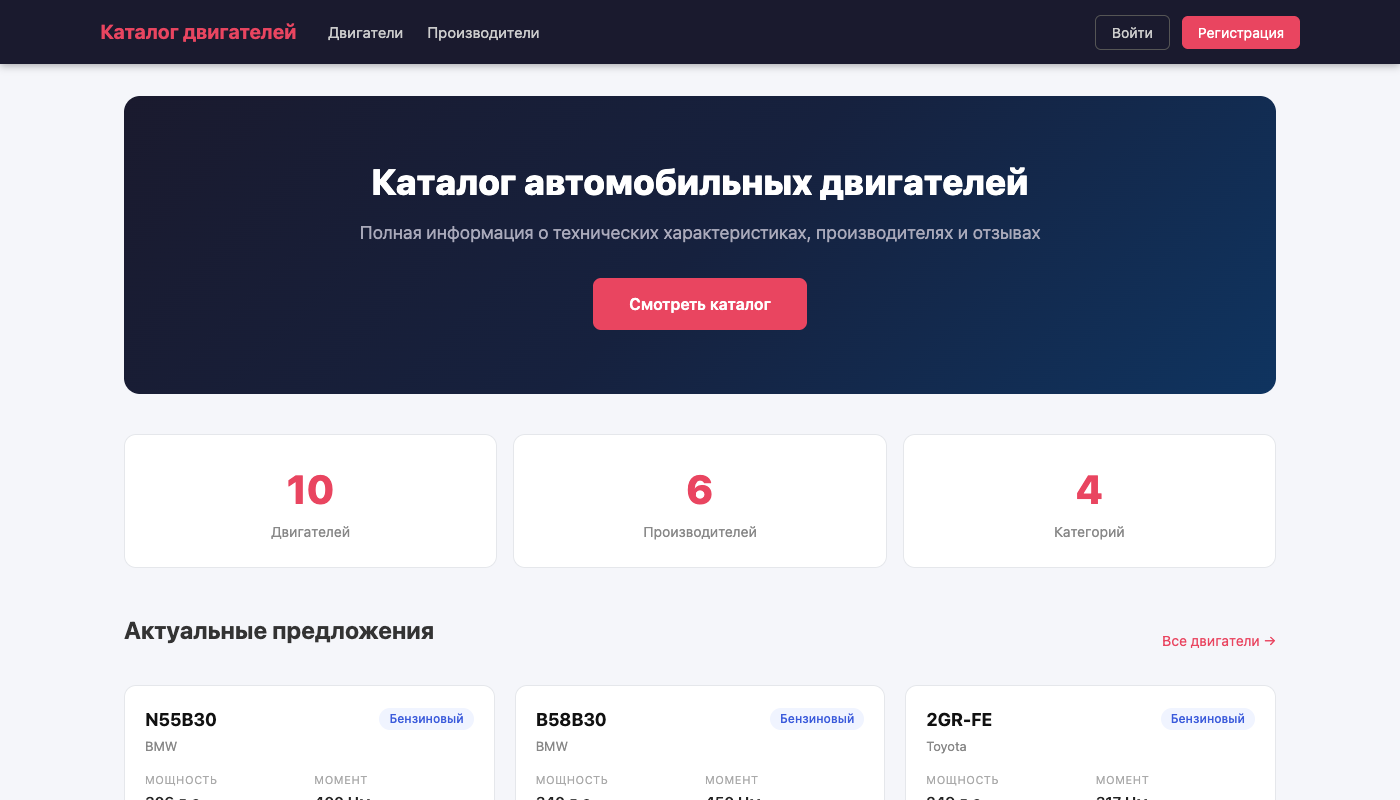
\includegraphics[width=\textwidth]{home.png}
  \caption{Главная страница приложения}
\end{figure}

На рисунке~7 показана страница каталога двигателей. Пользователю доступны поиск по названию, фильтрация по категории и производителю через выпадающие списки. Результаты отображаются в виде сетки карточек с ключевыми характеристиками.

\begin{figure}[h!]
  \centering
  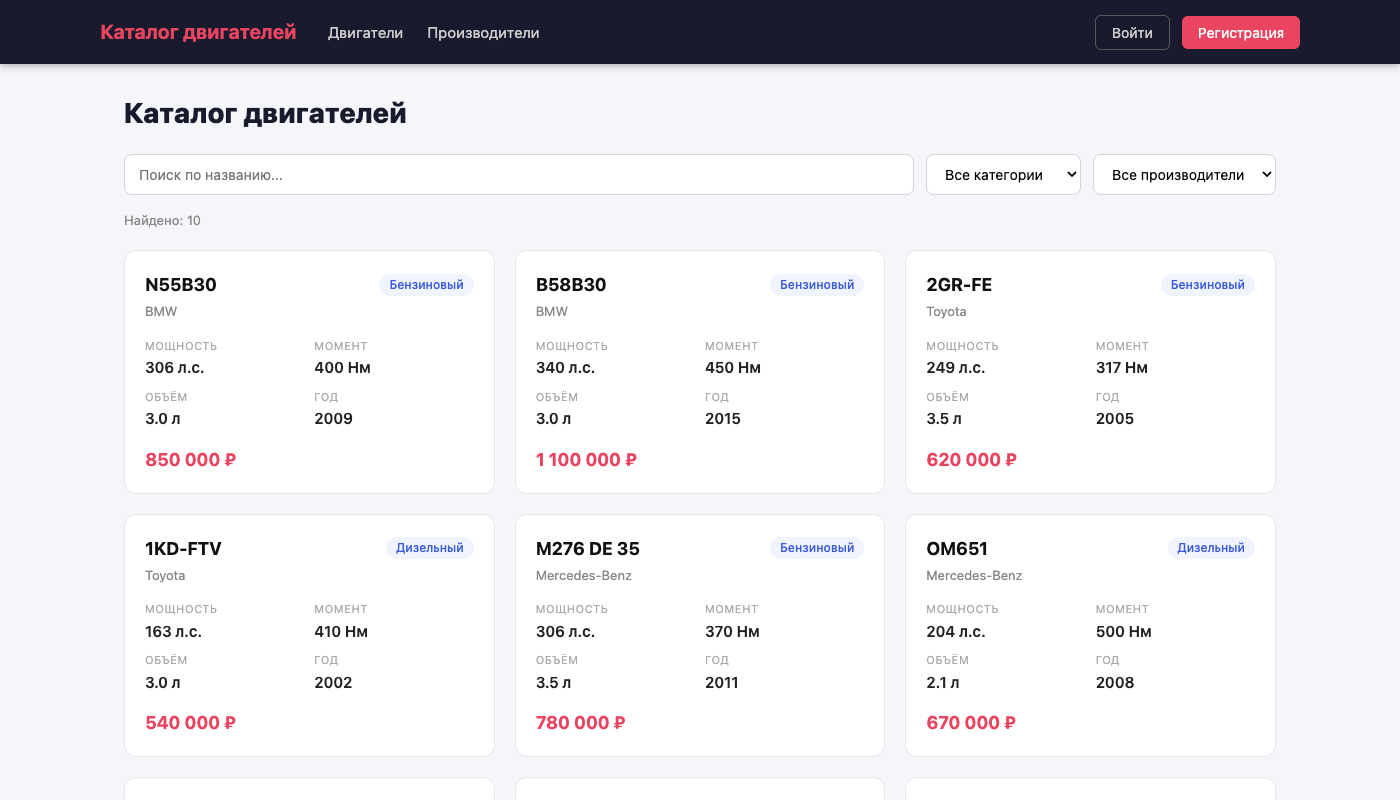
\includegraphics[width=\textwidth]{engines.png}
  \caption{Страница каталога двигателей}
\end{figure}

На рисунке~8 показана детальная страница двигателя. Левая часть содержит полную таблицу технических характеристик и описание. Правая часть --- список отзывов пользователей с оценками и форму добавления отзыва для авторизованных пользователей.

\begin{figure}[h!]
  \centering
  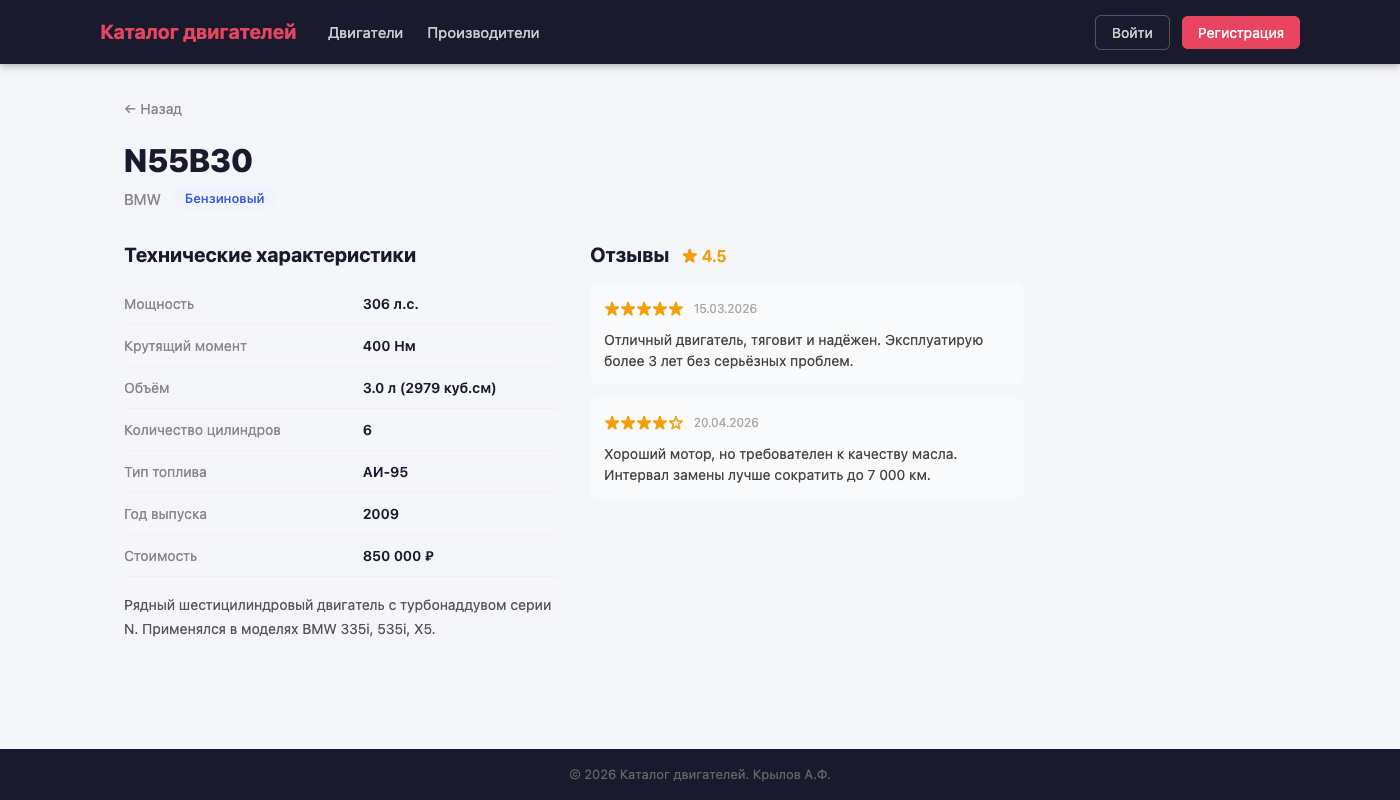
\includegraphics[width=\textwidth]{engine_detail.png}
  \caption{Детальная страница двигателя}
\end{figure}

На рисунке~9 представлена страница производителей с карточками компаний, указанием страны и года основания.

\begin{figure}[h!]
  \centering
  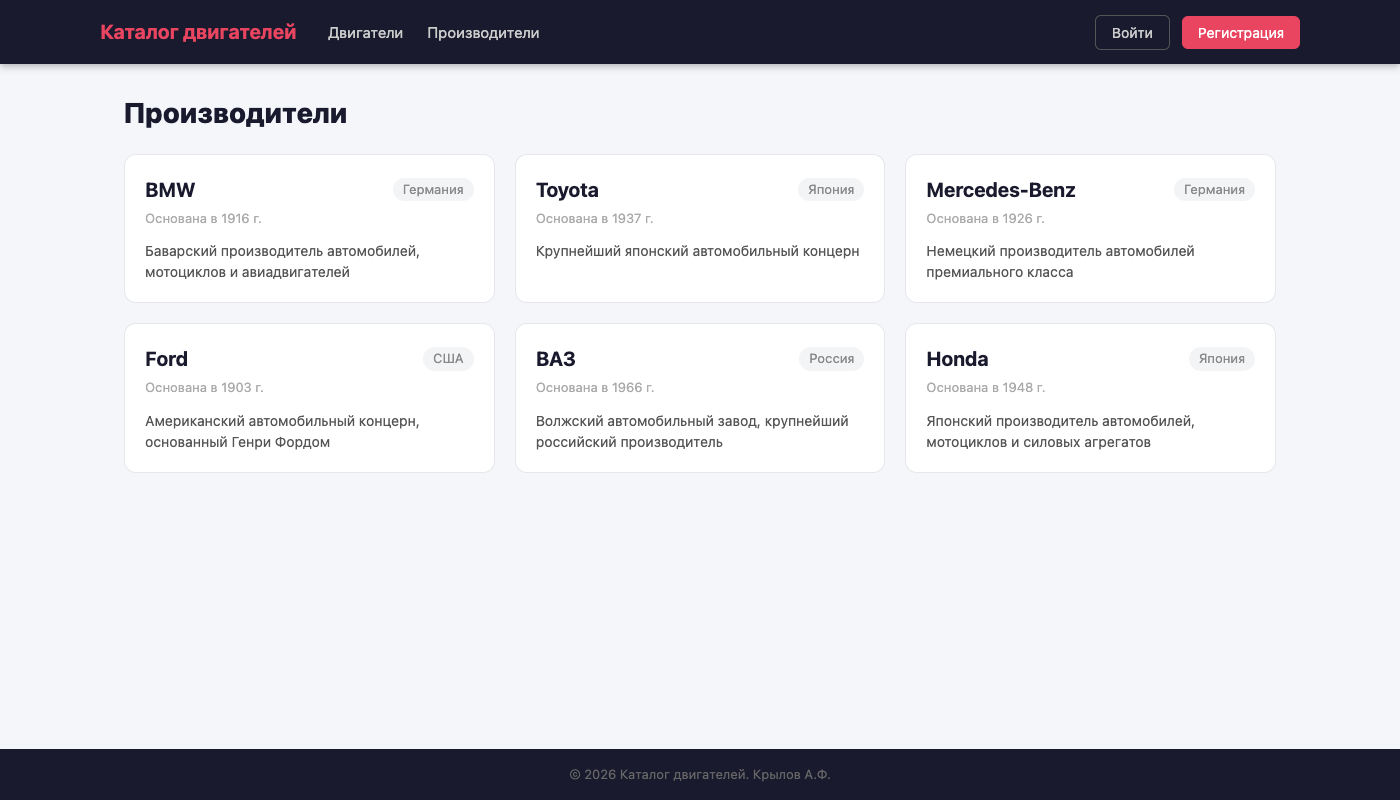
\includegraphics[width=\textwidth]{manufacturers.png}
  \caption{Страница производителей}
\end{figure}

На рисунке~10 представлена форма входа в систему. При успешной аутентификации JWT-токен сохраняется в \texttt{localStorage}, после чего пользователь перенаправляется на главную страницу.

\begin{figure}[h!]
  \centering
  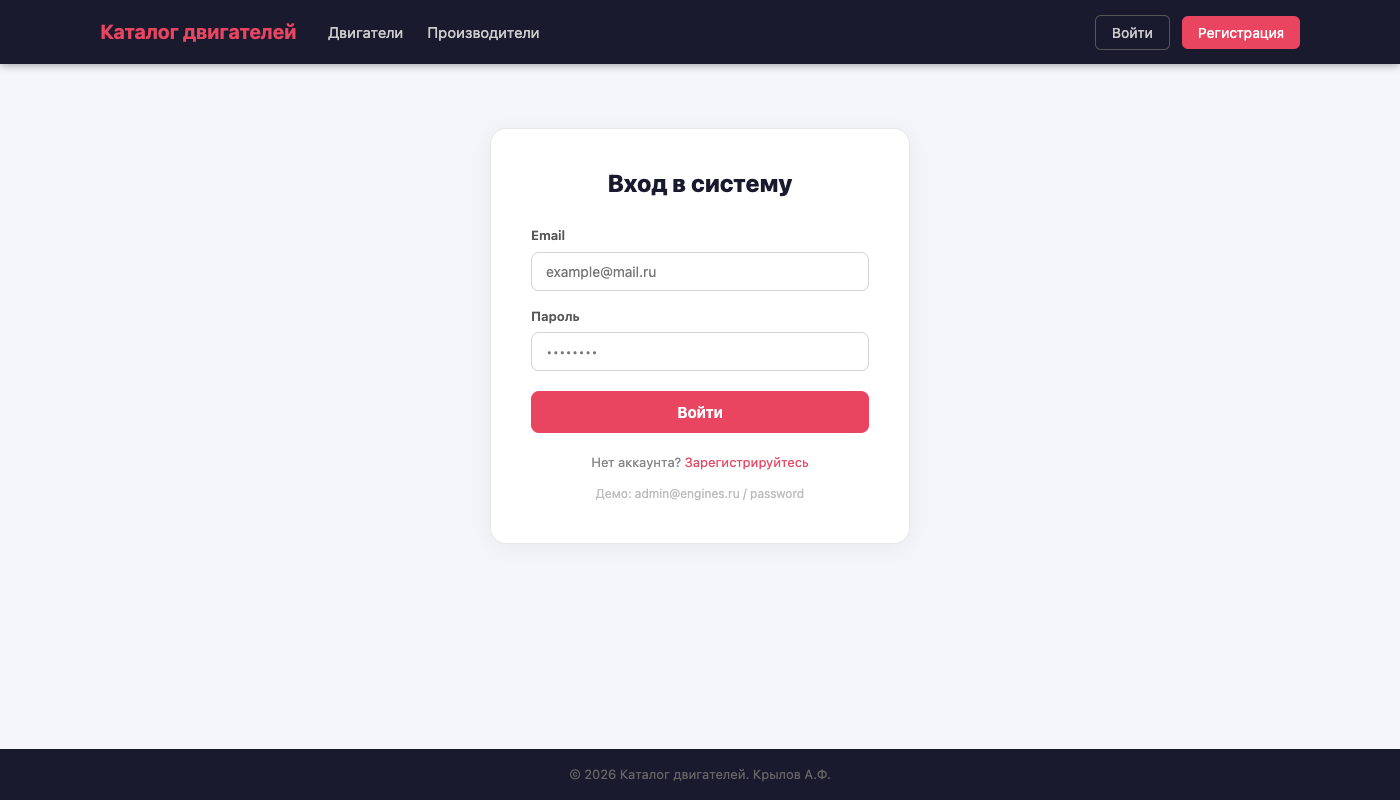
\includegraphics[width=\textwidth]{login.png}
  \caption{Страница входа в систему}
\end{figure}

На рисунке~11 представлена административная панель управления. Вкладки позволяют переключаться между управлением двигателями, производителями и категориями. Каждая вкладка содержит таблицу записей с кнопками редактирования и удаления, а также кнопку добавления новой записи.

\begin{figure}[h!]
  \centering
  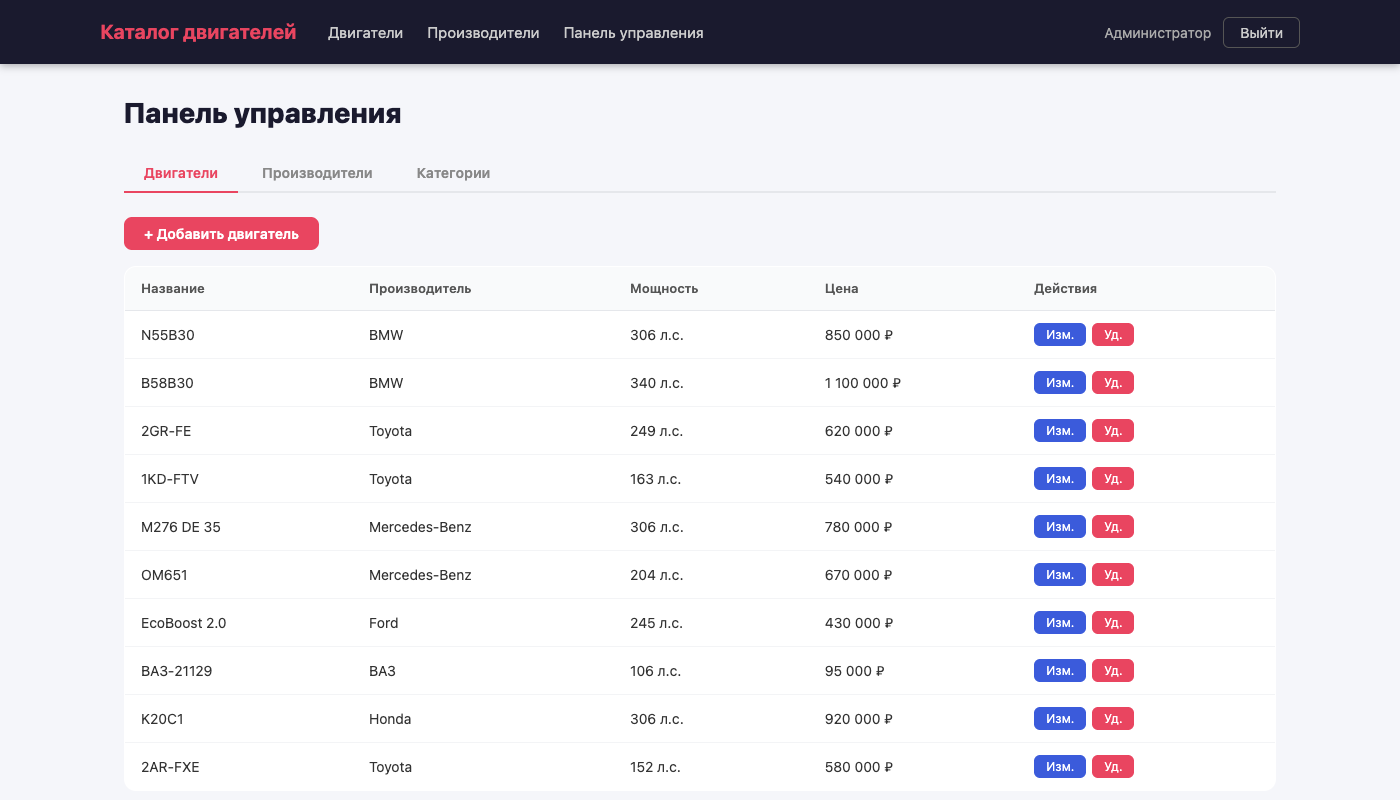
\includegraphics[width=\textwidth]{admin.png}
  \caption{Административная панель управления}
\end{figure}

\newpage

% ─── ПОРЯДОК ЗАПУСКА ───────────────────────────────────────────────────────────
\section{Порядок запуска приложения}

Для запуска приложения на локальной машине необходимо наличие установленных Node.js версии 18 и выше, а также менеджера пакетов npm.

\subsection{Запуск серверной части}

Перейти в директорию \texttt{backend} и выполнить следующие команды:

\begin{lstlisting}
npm install
npm run start:dev
\end{lstlisting}

Сервер запустится на порту~3000. В режиме разработки (\texttt{start:dev}) NestJS автоматически перезапускается при изменении исходных файлов.

\subsection{Запуск клиентской части}

В отдельном терминале перейти в директорию \texttt{frontend} и выполнить:

\begin{lstlisting}
npm install
npm run dev
\end{lstlisting}

Клиентское приложение будет доступно по адресу \texttt{http://localhost:5173}. Все запросы к \texttt{/api} автоматически проксируются на \texttt{http://localhost:3000} средствами Vite.

\subsection{Учётные данные для входа}

В таблице~9 приведены тестовые учётные записи, доступные после первого запуска.

\begin{table}[h!]
\caption{Тестовые учётные записи}
\begin{tabular}{|p{4.5cm}|p{3cm}|p{3cm}|p{3cm}|}
\hline
\textbf{Email} & \textbf{Пароль} & \textbf{Роль} & \textbf{Имя} \\
\hline
admin@engines.ru  & password & admin & Администратор \\
ivanov@mail.ru    & password & user  & Иванов И.И. \\
petrova@gmail.com & password & user  & Петрова А.С. \\
\hline
\end{tabular}
\end{table}

Данные каталога хранятся в JSON-файлах в директории \texttt{backend/data/} и не требуют инициализации базы данных. Все изменения, вносимые через административную панель, немедленно сохраняются в соответствующих файлах.

\newpage

% ─── ЗАКЛЮЧЕНИЕ ────────────────────────────────────────────────────────────────
\section{Заключение}

В рамках данной курсовой работы разработано клиент-серверное веб-приложение <<Каталог автомобильных двигателей>>. Предметная область включает рынок автомобильных силовых агрегатов, для которого характерна проблема разрозненности технической информации о характеристиках двигателей различных производителей и типов.

Разработанное приложение решает поставленную задачу: обеспечивает централизованное хранение и удобный доступ к каталогу двигателей с возможностью фильтрации по категории и производителю, детального просмотра технических характеристик, а также оценки агрегатов пользователями через систему отзывов.

В ходе работы реализованы все требования технического задания:
\begin{itemize}
  \item разграничение прав доступа по ролям (\texttt{user} / \texttt{admin});
  \item полный CRUD для двигателей, производителей и категорий;
  \item система отзывов с оценками от 1 до 5;
  \item JWT-аутентификация с хранением токена в \texttt{localStorage};
  \item все требуемые API-эндпоинты, включая \texttt{/users}, \texttt{/engines}, \texttt{/reviews} и \texttt{/auth/login};
  \item валидация входных данных на серверном уровне.
\end{itemize}

Использованные инструменты и технологии: NestJS~10 (серверный фреймворк), React~18 (клиентская библиотека), TypeScript~5, Vite~5 (сборщик), JSON-файлы (хранилище), JWT (аутентификация), bcrypt (хеширование паролей), class-validator (валидация), Axios (HTTP-клиент), React Router~6 (маршрутизация), CSS~Modules (стилизация).

Исходный код приложения доступен в git-репозитории~\cite{repo}.

\newpage

% ─── СПИСОК ЛИТЕРАТУРЫ ─────────────────────────────────────────────────────────
\begin{thebibliography}{8}

\bibitem{react}
React --- библиотека JavaScript для создания пользовательских интерфейсов. ---
URL: \url{https://react.dev} (дата обращения: 13.05.2026). --- Текст: электронный.

\bibitem{nestjs}
NestJS --- прогрессивный Node.js фреймворк. ---
URL: \url{https://docs.nestjs.com} (дата обращения: 13.05.2026). --- Текст: электронный.

\bibitem{typescript}
TypeScript --- типизированный JavaScript масштаба приложения. ---
URL: \url{https://www.typescriptlang.org/docs} (дата обращения: 13.05.2026). --- Текст: электронный.

\bibitem{jwt}
RFC~7519: JSON Web Token (JWT) / M.~Jones, J.~Bradley, N.~Sakimura. ---
Internet Engineering Task Force, 2015. ---
URL: \url{https://www.rfc-editor.org/rfc/rfc7519} (дата обращения: 13.05.2026). --- Текст: электронный.

\bibitem{passport}
Passport.js --- простая аутентификация для Node.js. ---
URL: \url{https://www.passportjs.org/docs} (дата обращения: 13.05.2026). --- Текст: электронный.

\bibitem{bcrypt}
Provos~N., Mazi\`eres~D. A Future-Adaptable Password Scheme /
N.~Provos, D.~Mazi\`eres // USENIX Annual Technical Conference. --- 1999. ---
URL: \url{https://www.usenix.org/legacy/event/usenix99/provos/provos.pdf}
(дата обращения: 13.05.2026). --- Текст: электронный.

\bibitem{vite}
Vite --- инструмент следующего поколения для фронтенд-разработки. ---
URL: \url{https://vite.dev} (дата обращения: 13.05.2026). --- Текст: электронный.

\bibitem{repo}
Крылов~А.Ф. Каталог автомобильных двигателей: исходный код проекта. ---
URL: \url{https://github.com/krylov-af/engine-catalog}
(дата обращения: 13.05.2026). --- Текст: электронный.

\end{thebibliography}

\end{document}
